\documentclass[a4paper,12pt]{scrartcl}
\usepackage[margin=2cm,bindingoffset=0cm]{geometry}
\usepackage{ucs}
\usepackage[utf8x]{inputenc}
\usepackage[ngerman]{babel}
\usepackage{fontenc}
%\usepackage[pdftex]{graphicx}
\usepackage{listings}
\usepackage{amssymb}
\usepackage{amsmath}
\usepackage{wasysym}
\usepackage{graphicx}
\usepackage[pdftex]{hyperref}
\author{Verena Käfer (2551188), Niklas Schnelle (2573250), Peter Vollmer (2553704)}
\date{erstellt am 15.11.2010\\
Version: 1.0}
\title{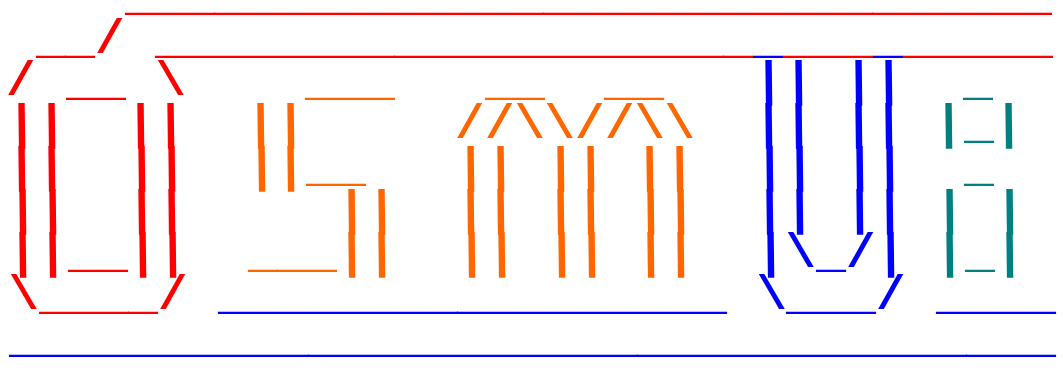
\includegraphics[width=15cm]{../projektplan/Logo_Osmui.png} \\ 
Spezifikation von OsmUi}

\begin{document}
\maketitle
\newpage
\tableofcontents
\newpage

\section{Einleitung}
\subsection{Zweck der Spezifikation}
Bei der Spezifikation handelt es sich um das zentrale Projektdokument. Sie ist Basis aller weiteren Dokumente und
Bezugspunkt in Funktionalitätsfragen. Sie ist daher unbedingt aktuell und konsistent zu halten.\\
Die Spezifikation beschreibt die Funktionen und Anforderungen an das Produkt OsmUi und das zugehörige Projekt.
\subsection{Leserkreis}
Diese Spezifikation richtet sich an:
\begin{itemize}
 \item Die Entwickler von OsmUi
 \item Den Kunden und die Betreuer des SoPra
\end{itemize}

\subsection{Projektüberblick}
In dem Entwicklungsprojekt OsmUi soll eine grafische Benutzeroberfläche für das Kommandozeilenwerkzeug \href{http://wiki.openstreetmap.org/wiki/Osmosis}{Osmosis}
entwickelt werden. Zu diesem Zweck überträgt OsmUi das abstrakte Pipelinekonzept von Osmosis auf eine grafische Darstellung, welche die gesamte Funktionalität von Osmosis zugänglich macht, dabei aber deutlich benutzerfreundlicher sein soll.\\
Während bei Osmosis ein langer Kommandozeilenaufruf eine Pipeline zur Verarbeitung von OpenStreetMap Daten beschreibt, wobei sich der Benutzer die Befehle merken
und korrekt in der gewünschten Reihenfolge aufschreiben muss, soll es mit OsmUi möglich sein eine Verarbeitungspipeline ``zusammen zu klicken''.\\
Hierbei kann die Funktionsweise der einzelnen Tasks sowie deren Interaktion der Benutzeroberfläche von OsmUi entnommen werden.
%\subsection{Konventionen} %Kommt noch

\section{Akteure}
\subsection{Benutzer}
Bei OsmUi gibt es grundsätzlich nur eine Nutzerklasse. Es wird davon ausgegangen, dass OsmUi benutzt wird um eine Verarbeitungspipeline für OpenStreetMap Daten
zu erstellen, welche anschließend durch Osmosis ``ausgeführt'' wird. Hierbei wird davon ausgegangen, dass der Nutzer grundlegende Kentnisse 
von Datenverarbeitung und OpenStreetMap hat.

\section{Distributionsform und Installation}
OsmUi wird als ausführbares JAR Archiv ausgeliefert, welches direkt ausgeführt werden kann

\section{Nichtfunktionale Anforderungen}
\subsection{Entwurfseinschränkungen}
\subsubsection{Entwurfskonzept}
OsmUi wird nach dem \href{http://de.wikipedia.org/wiki/KISS-Prinzip}{KISS-Prinzip} entwickelt, d.h. entscheidend für die Qualität der Software soll
sein, wie gut die Hauptfunktionen unterstützt werden. Bessere Hauptfunktionalität ist einem größeren Funktionsumfang unterzuordnen.\\
Im Fall von OsmUi heißt dies, dass das Hauptaugenmerk auf dem einfachen und sinnvollen Erstellen von Verarbeitungspipelines, sowie deren Import und Export liegt.\\
Weniger wichtig sind hingegen ``Luxusfunktionen'' wie direktes Anzeigen des Verarbeitungsergebnisses (was auf Grund der Vielfalt der Funktionen von Osmosis
und der Verarbeitungsdauer ohnehin nicht immer sinnvoll ist) oder das direkte Aufrufen von Osmosis.
\subsubsection{Systemumgebung}
Systemumgebung ist das \textbf{Java Runtime Environment in Version 1.6 und höher (SE)}. Dabei ist OsmUi als reine Java Anwendung zu entwickeln, so dass
keine externen Abhängigkeiten bestehen und OsmUi auf allen Java SE kompatiblen Systemen eingesetzt werden kann.
Eventuell wird intern die Bibliothek \textbf{JGraph} eingesetzt, diese wird dann aber direkt mit ausgeliefert
und ist ebenso in platformunabhängigem Java geschrieben. 
\subsubsection{Layout und Gestaltung}
OsmUi soll ab einer Auflösung von 1024x768 und bis zu einer Systemschriftgröße 24 benutzbar sein. Alle Fenster sollen, wenn dies sinnvoll ist, skalierbar sein und den eventuell gewonnenen Platz
nutzen. Um Benutzer von Multimonitorsystemen und exotischen Windowmanagern zu entlasten soll die Positionierung von neuen Fenstern nativ erfolgen. Es
sollen insbesondere keine Fenster in eine errechnete Bildschirmmitte von OsmUi positioniert werden.
\subsection{Robustheit}
OsmUi soll als Software möglichst robust arbeiten, d.h. unter allen Bedingungen korrekt arbeiten. Dies soll durch defensive Programmierung erreicht werden.
Jedoch sollen Benutzereingaben möglichst früh geprüft werden, so dass tiefere Funktionen den Daten ``vertrauen'' können. Dies sichert zudem ab, dass klar ist, welcher
Programmteil für die Prüfung zuständig ist. Nämlich immer der erste, der die nötigen Informationen hat.\\
Weiterhin wird die Robustheit durch das KISS-Prinzip unterstützt, da weniger Funktionen besser entworfen und getestet werden können.
\subsection{Portabilität}
OsmUi soll durch den Einsatz reinen Javas auf allen Systemen mit Java SE 1.6 Unterstützung lauffähig sein. Als Exportformate für Osmosis Aufrufskripte
werden .bat und .sh (/bin/sh) unterstützt, womit alle Posix Systeme sowie Windows abgedeckt sind.
\subsection{Erweiterbarkeit}
Das Programm muss keine besonderen Erweiterungsfunktionalitäten wie etwa ein Pluginsystem zur Verfügung stellen, jedoch werden der Programmcode und die Systemarchitektur
so gestaltet, dass OsmUi leicht und schnell an neue oder veränderte Osmosis Funktionen angepasst werden kann.



\section{Funktionale Anforderungen}
\subsection{Mengengerüst}
Bei OsmUi handelt es sich um eine Einzelplatzanwendung und es wird keine Netzwerkfunktion genutzt, somit gibt es zu jedem Zeitpunkt genau einen Nutzer.\\
Beim Erstellen/Laden/Speichern von Verarbeitungspipelines muss OsmUi in der Lage sein, mit Pipelines von bis zu 100 Tasks zuverlässig zu arbeiten -
eine künstliche Beschränkung nach oben besteht jedoch nicht.\\
Werden 100 Tasks nicht überschritten und das System des Nutzers nicht unnormal ausgelastet, so muss OsmUi Benutzeraktionen, wie laden/speichern, task hinzufügen etc.
innerhalb von 1 Sekunde ausführen. Hierbei darf ein Mittelklasserechner angenommen werden. (>= 2.6 Ghz, >= 1 GB RAM, 7200 RPM Festplatte)
\subsection{persistente Konfiguration}
Um Benutzerspezifische Einstellungen zu speichern verwendet OsmUi eine Konfigurationsdatei im Heimat-/Configverzeichnis des Benutzters.
Diese Konfigurationsdatei wird ein für Menschen lesbaren XML Format gespeichert, wobei die genaue Definition in der Entwurf- bzw. Implementierungsphase
spezifiziert wird. 
\subsection{Laden und Speichern in OsmUi eigenem Format}
Um Pipelines mit allen Details wie Position von verschobenen Tasks, sowie nicht ausführbare Pipelines speichern zu können verwendet OsmUi ein eigenes Dateiformat
(.smu) außerdem ist dieses Format plattformunabhängig.
\subsection{Importieren und Exportieren von Verarbeitungspiplines aus Osmosis Aufrufen}
Um mit anderen Osmosis Oberflächen und bereits gesammelten Osmosis Aufrufen kompatibel zu bleiben bietet OsmUi verschiedene Im- und Export Funktionen
\subsubsection{Importieren von Osmosis Aufrufen}
OsmUi kann Osmosis Aufrufe beziehungsweise Parameterlisten der Form `--read-xml foo.osm --bb left=8 right=8.4 top=49 bottom=48 --write-xml bar.osm'' 
importieren, dabei stehen folgende Möglichkeiten der Eingabe zur Verfügung
\begin{itemize}
  \item Aus Zwischenablage\\
  Beim Importieren aus der Zwischenablage wird der Osmosis Aufruf (s.o.) direkt aus der Zwischenablage gelesen und die Pipeline geladen.
  \item Aus Aufrufskripten\\
  Hierbei liest OsmUi den Osmosis Aufruf aus einem Aufrufskript, es werden sowohl .bat Dateien, als auch .sh Dateien unterstützt.
\end{itemize}
\subsubsection{Exportieren}
OsmUi kann Pipelines als Aufrufskript im .sh Format (mit \#!/bin/sh Shebang) für alle Posix Konformen Systeme, sowie im .bat Format für Windows exportieren.
Der Pfad mit dem Osmosis aufgerufen wird, kann dabei vom Benutzer eingestellt werden. Falls dieser zu einer .jar Datei zeigt wird ``java -jar '' davor
gehängt.\\ 
Neben dem speichern als fertiges Aufrufskript, kann der Osmosis Aufruf auch aus der Kopierleiste kopiert werden
um ihn zum Beispiel in andere Dokumente einzubinden. 

\subsection{Benutzeroberfläche}
Die Benutzeroberfläche von OsmUi ist in zwei Teile aufgeteilt: die Taskpalette und die Pipelinebox. Desweiteren gibt es ein Anwendungsmenü und beim Bearbeiten eines Tasks
wird es ein weiteres Einstellungsfenster geben.\\
\begin{center}
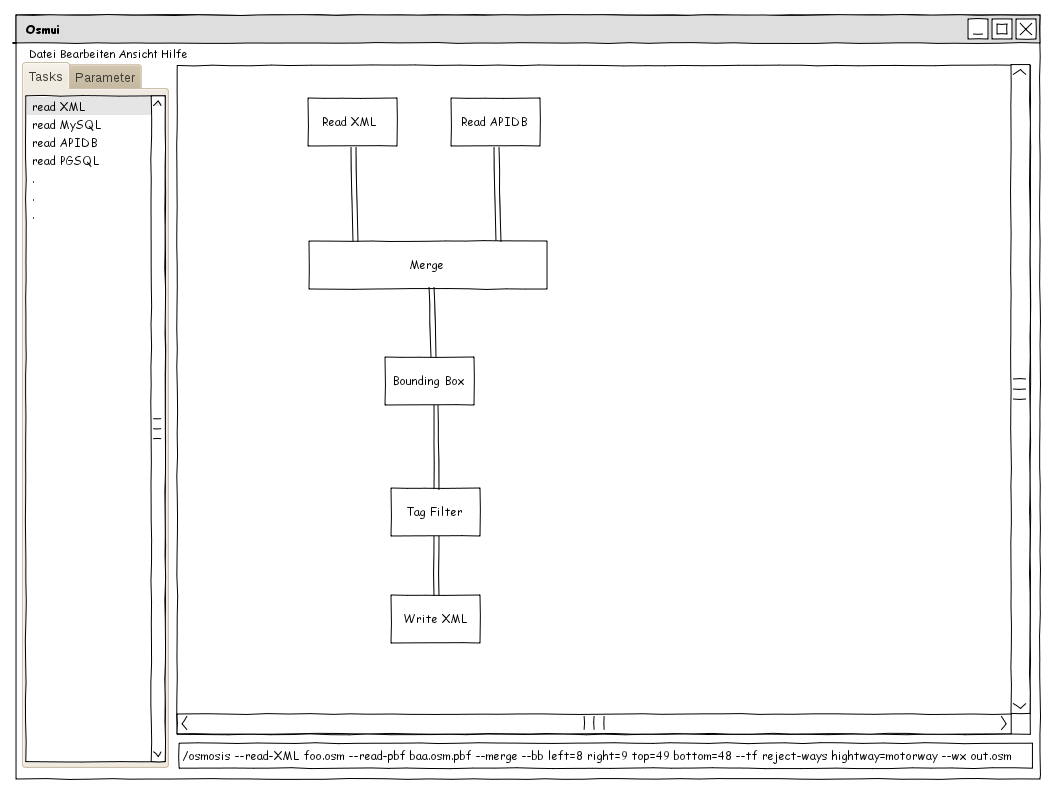
\includegraphics[width=15cm]{ui_prototype/OsmUi_Startseite.png}
\end{center}
\subsubsection{Taskpalette (Tasktab)}
Im linken Teil der Benutzeroberfläche wird Tasktab eine Liste der gerade zum Einfügen verfügbaren Tasks dargestellt. Dabei kann die Darstellung als Icon,
Text oder Kombination erfolgen. Es werden nur Tasks angezeigt die gerade auch einfügbar sind. \\
Am Anfang sind dies zum Beispiel alle Tasks, (z.B. read XML) die keinen Streameingang haben. Ist in der Pipelinebox ein Task ausgewählt, so
sind nur diejenigen Tasks sichtbar, die mit dem/den Ausgang/Ausgängen des ausgewählten Task kompatibel sind.\\
So wird verhindert, dass der Benutzer Pipelines bauen kann, die nicht durch Osmosis ausführbar sind.
\subsubsection{Pipelinebox}
In der Pipelinebox wird die Pipeline grafisch dargestellt und es können Tasks zum Bearbeiten ausgewählt werden. Ist ein Task ausgewählt so können seine Eigenschaften
bearbeitet oder ein neuer Task über die Taskpalette - wie oben beschrieben - angefügt werden. Desweiteren kann eine Verbindung zu einem anderen Task, der noch offene
Inputs hat, hergestellt werden.
\subsubsection{Parametertab}
Wählt der Benutzer einen Task aus, so zeigt OsmUi den Parametertab an, in dem alle - für den jeweiligen Tasktyp vorhandenen - Parameter eingegeben werden können.
Hierbei kann die Eingabe eingeschränkt sein und als Spanne von Zahlen, als Kartenausschnitt oder als freier Text erfolgen. Dabei wird der für
den Datentyp beste Eingabemodus gewählt.\\
\begin{center}
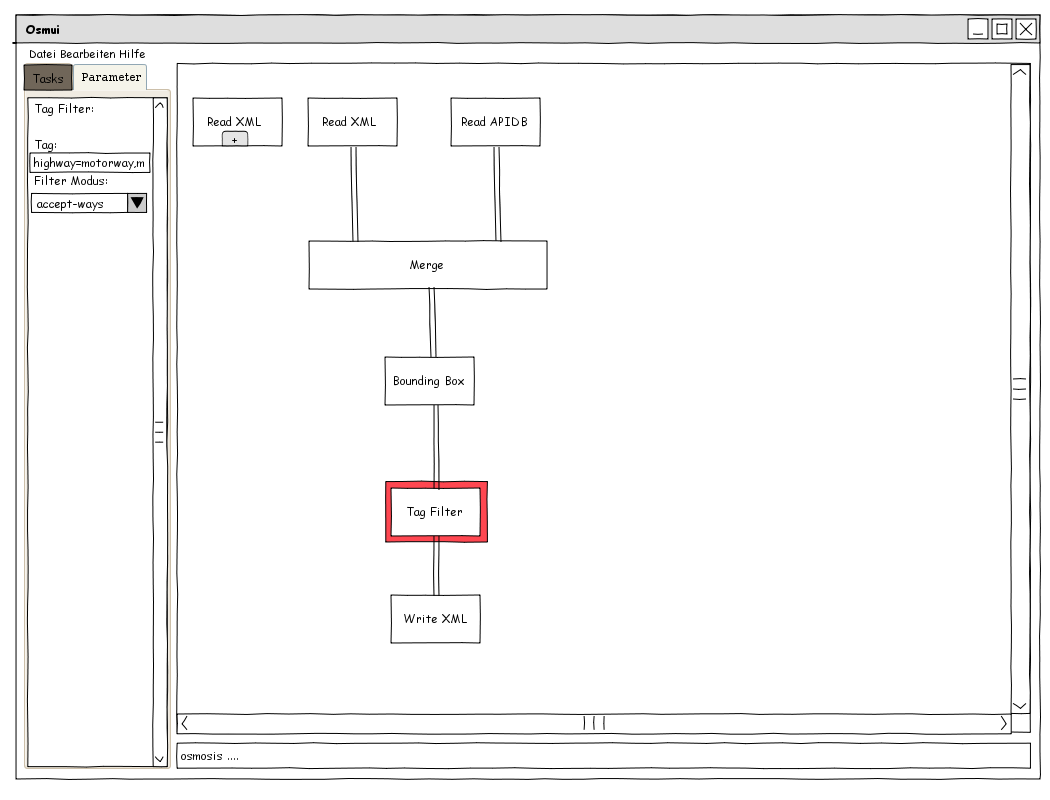
\includegraphics[width=15cm]{ui_prototype/OsmUi_Parameter_Optionen.png}
\end{center}
\subsubsection{Optionsdialog}
Im Einstellungsdialog können Benutzerspezifische Einstellungen von OsmUi vorgenommen werden, welche persistent in einer Konfigurationsdatei gespeichert werden.\\
Hierzu zählen:\\
\begin{itemize}
 \item Einstellung des Pfades zu Osmosis, welcher in Aufrufskripten verwendet werden soll
\end{itemize}


\subsubsection{Kopierleiste}
Um die aktuell dargestellte Pipeline direkt kopieren zu können, wird sie als Osmosis-Aufruf unter der Pipelinebox angezeigt.
\begin{center}
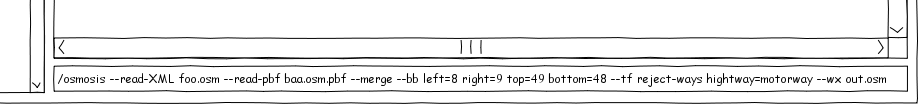
\includegraphics[width=15cm]{ui_prototype/OsmUi_Leisteklein.png}
\end{center}

\subsubsection{Menüleiste}
\begin{itemize}
\item Datei\\
Beim Klicken auf den Menüeintrag \textbf{Datei} öffnet sich ein Dialog. Der Benutzer kann zwischen \textbf{Neu} (Öffnen einer neuen Pipeline), \textbf{Laden...} (Laden einer gespeicherten Datei), \textbf{Speichern} (automatisches speichern der aktuellen Pipeline), \textbf{speichern unter} (speichern der vorhandenen Datei an einem selbst gewählten Ort) und \textbf{schließen} (das Programm wird geschlossen) wählen. 
\\ 
\begin{center}
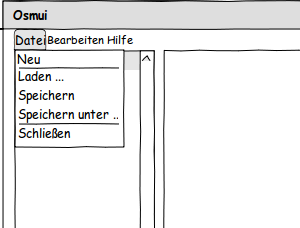
\includegraphics[width=7cm]{ui_prototype/OsmUi_Dateiklein.png}
\end{center}
\item Bearbeiten\\
Beim Klicken auf den Menüeintrag \textbf{Bearbeiten} öffnet sich ein Dialog. Der Benutzer kann zwischen \textbf{Rückgängig} (die letzte Änderung wird wieder rückgängig gemacht) und \textbf{wiederherstellen} (eine rückgängig gemachte Änderung wird wieder hergestellt) wählen.
\\
\begin{center}
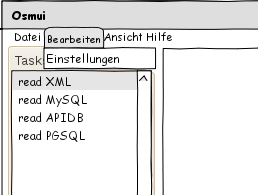
\includegraphics[width=7cm]{ui_prototype/OsmUi_Bearbeitenklein.png}
\end{center}
\item Hilfe\\
Beim Klicken auf den Menüeintrag \textbf{Hilfe} öffnet sich ein Dialog. Der Benutzer kann zwischen \textbf{Hilfe} (Onlinehilfe wird geöffnet) und \textbf{Über...} (Informationen zu OsmUi werden geöffnet) entscheiden.
\\
\begin{center}
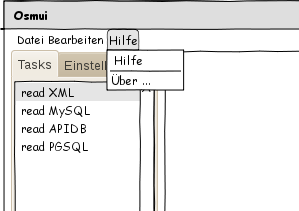
\includegraphics[width=7cm]{ui_prototype/OsmUi_Hilfeklein.png}
\end{center}
\end{itemize}

\subsubsection{Lokalisation}
OsmUi wird eine übersetzte Benutzeroberfläche für mindestens die Sprachen Deutsch und Englisch bieten. Dabei wird die aktuell verwendete
Sprache aus den hierfür vorgesehenen Umgebungsvariablen eingelesen, um sie ohne Interaktion durch den Benutzer in dessen System einzugliedern.
\newpage
\section{Use Cases}
\subsection{Diagramm}
\begin{center}
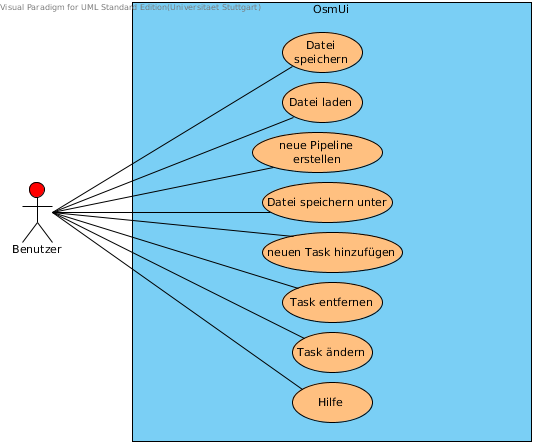
\includegraphics[width=15cm]{Use-Cases.png}
\end{center}
\subsection{Beschreibungen}
\begin{center}
\ \\
\begin{tabular}{|p{5cm}|p{10cm}|}
\hline Name & \textbf{Datei laden} \\ 
\hline Ziel & gespeicherte Daten in OsmUi anzuzeigen \\ 
\hline Vorbedingung & Eine gespeicherte Datei ist vorhanden \\
\hline Nachbedingung & Die Datei wurde geladen und zeigt die Pipeline an\\ 
\hline Nachbedingung im Sonderfall 5a) & OsmUi hat keine Daten geladen und zeigt Zustand vor dem Ladeversuch \\ 
\hline Nachbedingung im Sonderfall 6a) & OsmUi hat keine Daten geladen und zeigt Zustand vor dem Ladeversuch \\ 
\hline Nachbedingung im Sonderfall 7a) & Daten wurden geladen\\
\hline Nachbedingung im Sonderfall 7b) & OsmUi hat keine Daten geladen und zeigt Zustand vor dem Ladeversuch \\
\hline Nachbedingung im Sonderfall 7c) & OsmUi hat keine Daten geladen und zeigt Zustand vor dem Ladeversuch \\
\hline Nachbedingung im Sonderfall 7d) & OsmUi hat keine Daten geladen und zeigt Zustand vor dem Ladeversuch \\
\hline Akteure & Benutzer \\ 
\hline Normalablauf & 1 Der Benutzer klickt auf Datei.
\newline 2 OsmUi zeigt den Menüeintrag Datei
\newline 3 Der Benutzer klickt auf Datei laden.
\newline 4 OsmUi zeigt den Dateiauswahldialog
\newline 5 Der Benutzer wählt die gewünschte Datei aus
\newline 6 Der Benutzer bestätigt dies mit Klick auf Button ''Öffnen''.
\newline 7 OsmUi lädt die Datei und zeigt sie in der Piplinebox an\\ 
\hline Sonderfall 5a) & 5a.1 Der Benutzer klickt auf ''Abrechen''
\newline 5a.2 OsmUi lädt keine Daten und zeigt den vorherigen Zustand.\\
\hline Sonderfall 6a) & 6a.1 Der Benutzer klickt aber auf ''Abrechen''
\newline 6a.2 Osmui lädt keine Daten und zeigt den vorherigen Zustand.\\
\hline Sonderfall 7a) & Pipelinebox ist nicht leer.
\newline 7a.1 Osmui lädt die Datei in die Piplinebox einer neuen Instanz von OsmUi.\\
\hline Sonderfall 7b)& Datei ist zwischenzeitlich nicht mehr verfügbar.
\newline 7b.1 OsmUi versucht Datei zu lesen bricht dann ab und zeigt einen entsprechenden Fehlerdialog an.
\newline 7b.2 Benutzer klickt auf Button ''Ok''.
\newline $ \rightarrow$ Schritt 4\\
\hline Sonderfall 7c)& Benutzer besitzt keine Leserechte zur ausgewählten Datei.
\newline $ \rightarrow$ Schritt 7b.1 \\
\hline Sonderfall 7d)& Dateityp wird nicht unterstützt.
\newline $ \rightarrow$ Schritt 7b.1 \\
\hline 
\end{tabular} 
\vspace{0.7cm}
\\
\begin{tabular}{|p{5cm}|p{10cm}|}
\hline Name & \textbf{Datei speichern} \\ 
\hline Ziel & Aktuelle Datei soll gespeichert werden \\ 
\hline Vorbedingung & Die aktuelle Datei wurde schon einmal gespeichert \\ 
\hline Nachbedingung & Die Datei wurde gespeichert \\ 
\hline Nachbedingung im Sonderfall & Die Datei wurde gespeichert \\ 
\hline Akteur & Benutzer \\ 
\hline Normalablauf & 1 Der Benutzer klickt auf Datei
\newline 2 OsmUi zeigt den Menüeintrag Datei
\newline 3 Der Benutzer klickt auf Datei speichern
\newline 4 Die Datei wird gespeichert\\
\hline Sonfall 4a) & Die Datei wurde noch nie gespeichert
\newline 4a.1 $ \rightarrow$ Use Case Speichern unter Schritt 1\\
\hline 
\end{tabular}
\vspace{0.7cm}
\\
\begin{tabular}{|p{5cm}|p{10cm}|}
\hline Name & \textbf{Datei speichern unter} \\ 
\hline Ziel & Die Datei soll in einem selbst gewählten Verzeichnis gespeichert werden \\ 
\hline Vorbedingung & keine \\ 
\hline Nachbedingung & Die Datei wurde im gewählten Verzeichnis gespeichert\\ 
\hline Nachbedingung im Sonderfall 5a)& Die Datei wurde nicht gespeichert\\ 
\hline Nachbedingung im Sonderfall 5b)& Die Datei wurde nicht gespeichert\\
\hline Nachbedingung im Sonderfall 6a)& Die Datei wurde nicht gespeichert\\ 
\hline Akteur & Benutzer \\ 
\hline Normalablauf & 1 Der Benutzer klickt auf Datei
\newline 2 OsmUi zeigt den Menüeintrag Datei
\newline 3 Der Benutzer klickt auf Datei speichern unter
\newline 4 OsmUi zeigt den Dateiauswahldialog
\newline 5 Der Benutzer wählt den gewünschten Namen und die Dateiendung aus
\newline 6 Der Benutzer bestätigt dies mit Klick auf den Button ''Speichern'' 
\newline 7 Die Datei wird gespeichert\\
\hline Sonderfall 5a) & 5a.1 Der Benutzer klickt auf Abbrechen\\
\hline Sonderfall 5b) & 5b.1 Der Benutzer klickt auf eine bereits vorhandene Datei
\newline 5b.2 OsmUi fragt, ob die Datei überschrieben werden soll
\newline 5b.3 Der Benutzer klickt auf Ja
\newline 5b.4 Die Datei wird gespeichert\\
\hline Sonderfall 5b3a) & 5b3a.1 Der Benutzer klickt auf Nein
\newline $ \rightarrow$ Schritt 5\\
\hline Sonderfall 6a) & 6a.1 Der Benutzer klickt auf abbrechen\\
\hline 
\end{tabular}
\vspace{0.7cm}
\\
\begin{tabular}{|p {5cm}|p{10cm}|}
\hline Name & \textbf{aus Aufrufskript importieren}\\
\hline Ziel & importierte Datei soll angezeigt werden\\
\hline Vorbedingung & Eine importierbare Datei ist vorhanden\\
\hline Nachbedingung & Die Datei wurde importiert und die Pipeline angezeigt\\ 
\hline Nachbedingung im Sonderfall 5a) & OsmUi hat keine Daten importiert und zeigt Zustand vor dem Importversuch \\ 
\hline Nachbedingung im Sonderfall 6a) & OsmUi hat keine Daten importiert und zeigt Zustand vor dem Importversuch \\ 
\hline Nachbedingung im Sonderfall 7a) & Daten wurden importiert\\
\hline Nachbedingung im Sonderfall 7b) & OsmUi hat keine Daten importiert und zeigt Zustand vor dem Importversuch \\
\hline Nachbedingung im Sonderfall 7c) & OsmUi hat keine Daten importiert und zeigt Zustand vor dem Importversuch \\
\hline Nachbedingung im Sonderfall 7d) & OsmUi hat keine Daten importiert und zeigt Zustand vor dem Importversuch \\
\hline Akteure & Benutzer \\ 
\hline Normalablauf & 1 Der Benutzer klickt auf Datei.
\newline 2 OsmUi zeigt den Menüeintrag Datei
\newline 3 Der Benutzer klickt auf Importieren aus Datei
\newline 4 OsmUi zeigt den Dateiauswahldialog
\newline 5 Der Benutzer wählt die gewünschte Datei aus
\newline 6 Der Benutzer bestätigt dies mit Klick auf Button ''Importieren''.
\newline 7 OsmUi importiert die Datei und zeigt sie in der Piplinebox an.\\ 
\hline Sonderfall 5a) & 5a.1 Der Benutzer klickt auf ''Abrechen''
\newline 5a.2 OsmUi lädt keine Daten und zeigt den vorherigen Zustand.\\
\hline Sonderfall 6a) & 6a.1 Der Benutzer klickt aber auf ''Abrechen''
\newline 6a.2 Osmui importiert keine Daten und zeigt den vorherigen Zustand.\\
\hline Sonderfall 7a) & Pipelinebox ist nicht leer.
\newline 7a.1 Osmui importiert die Datei in die Piplinebox einer neuen Instanz von OsmUi.\\
\hline Sonderfall 7b)& Datei ist zwischenzeitlich nicht mehr verfügbar.
\newline 7b.1 OsmUi versucht Datei zu lesen bricht dann ab und zeigt einen entsprechenden Fehlerdialog an.
\newline 7b.2 Benutzer klickt auf Button ''Ok''.
\newline $ \rightarrow$ Schritt 4\\
\hline Sonderfall 7c)& Benutzer besitzt keine Leserechte zur ausgewählten Datei.
\newline $ \rightarrow$ Schritt 7b.1 \\
\hline Sonderfall 7d)& Dateityp wird nicht unterstützt.
\newline $ \rightarrow$ Schritt 7b.1 \\
\hline 
\end{tabular}
\vspace{0.7cm}
\\
\begin{tabular}{|p {5cm}|p{10cm}|}
\hline Name & \textbf{rückgängig machen} \\ 
\hline Ziel & der letzte Schritt soll Rückgängig gemacht werden\\
\hline Vorbedingung & Es muss mindestens ein Schritt gemacht worden sein\\
\hline Nachbedingung & Der Schritt wurde Rückgängig gemacht\\
\hline Akteur & Benutzer\\
\hline Normalablauf & 1 Der Benuzer klickt auf den Menüeintrag Bearbeiten
\newline 2 OsmUi öffnet das Bearbeiten Menü
\newline 3 Der Benutzer klickt auf Rückgängig
\newline 4 Der letzte Schritt wird rückgängig gemacht\\
\hline 
\end{tabular}
\vspace{0.7cm}
\\
\begin{tabular}{|p {5cm}|p{10cm}|}
\hline Name & \textbf{wiederherstellen} \\ 
\hline Ziel & der letzte Schritt soll wieder hergestellt werden werden\\
\hline Vorbedingung & Es muss mindestens ein Schritt rückgängig gemacht worden sein\\
\hline Nachbedingung & Der Schritt wurde wiederhergestellt gemacht\\
\hline Akteur & Benutzer\\
\hline Normalablauf & 1 Der Benuzer klickt auf den Menüeintrag Bearbeiten
\newline 2 OsmUi öffnet das Bearbeiten Menü
\newline 3 Der Benutzer klickt auf wiederherstellen
\newline 4 Der letzte Schritt wird wiederhergestellt\\
\hline 
\end{tabular}
\vspace{0.7cm}
\\
\begin{tabular}{|p {5cm}|p{10cm}|}
\hline Name & \textbf{Hilfe aufrufen} \\ 
\hline Ziel & Der Hilfe-Dialog soll aufgerufen werden \\ 
\hline Vorbedingung & keine \\ 
\hline Nachbedingung & Dem Benutzer wurde geholfen \\ 
\hline Nachbedingung im Sonderfall 5a) & Dem Benutzer wurde geholfen\\
\hline Nachbedingung im Sonderfall 5b) & Keine Hilfe wurde gegeben\\
\hline Nachbedingung im Sonderfall 7a) & Dem Benutzer wurde geholfen\\
\hline Akteur & Benutzer \\ 
\hline Normalablauf & 1 Der Benutzer klickt auf Hilfe
\newline 2 OsmUi zeigt den Menüeintrag Hilfe
\newline 3 Der Benutzer klickt auf Hilfe
\newline 4 OsmUi öffnet die Onlinehilfe
\newline 5 Der Benutzer klickt auf das gesuchte Stichwort
\newline 6 OsmUi zeigt den entsprechenden Eintrag
\newline 7 Der Benutzer klickt auf ''schließen''\\ 
\hline Sonderfall 5a) & 5a.1 Der Benutzer gibt einen Suchbegriff in die Suchleiste ein
\newline 5a.2 Der Benutzer bestätigt die Suche
\newline 5a.3 OsmUi zeigt alle Einträge an, die das/die Wort/Wörter enthält
\newline $ \rightarrow$ Schritt 5\\
\hline Sonderfall 5a2a) & $ \rightarrow$ Schritt 5\\
\hline Sonderfall 5a2b) & $ \rightarrow$ Schritt 5b\\
\hline Sonderfall 5b) & 5b.1 der Benutzer klickt auf ''schließen''
\newline 5b.2 OsmUi schließt das Menü\\
\hline Sonderfall 7a) & $ \rightarrow$ Schritt 5\\
\hline
\end{tabular}
\vspace{0.7cm}
\\
\begin{tabular}{|p{5cm}|p{10cm}|}
\hline Name & \textbf{Hilfe-über aufrufen} \\ 
\hline Ziel & Informationen über OsmUi einholen\\
\hline Vorbedingung & keine\\
\hline Nachbedingung & die Informationen wurden angezeigt\\
\hline Akteur & Benutzer\\
\hline Normalablauf & 1 Der Benutzer klickt auf Hilfe
\newline 2 OsmUi zeigt den Menüeintrag Hilfe
\newline 3 Der Benutzer klickt auf über
\newline 4 OsmUi öffnet die Informationsseite zu OsmUi
\newline 5 Der Benutzer klickt ausf Schließen\\
\hline
\end{tabular}
\vspace{0.7cm}
\\
\begin{tabular}{|p{5cm}|p{10cm}|}
\hline Name & \textbf{neue Pipeline erstellen} \\ 
\hline Ziel & Eine neue Pipeline soll erstellt werden \\ 
\hline Vorbedingung & keine \\ 
\hline Nachbedingung & Eine neues OsmUi Fenster mit leerer Pipeline wurde erstellt \\ 
\hline Akteur & Benutzer \\ 
\hline Normalablauf & 1 Der Benutzer klickt auf bearbeiten
\newline 2 OsmUi zeigt den Menüeintrag bearbeiten
\newline 3 Der Benutzer klickt auf neu
\newline 4 Ein neue Instanz von OsmUi mit leerer Pipeline wird gestartet\\ 
\hline 
\end{tabular} 
\vspace{0.7cm}
\\
\begin{tabular}{|p{5cm}|p{10cm}|}
\hline Name & \textbf{neuen Task hinzufügen} \\ 
\hline Ziel & Ein neuer Task soll hinzugefügt werden \\ 
\hline Vorbedingung& keine \\
\hline Nachbedingung & Ein neuer Task wurde hinzugefügt \\ 
\hline Nachbedingung im Sonderfall 1a) & Ein neuer Input-Task wurde unverbunden hinzugefügt\\
\hline Nachbedingung im Sonderfall 1b) & Kein neuer Task wurde hinzugefügt\\
\hline Akteur & Benutzer \\ 
\hline Normalablauf & 1 Der Benutzer klickt auf einen Plus-Button des Tasks (bei mehreren Ausgängen gibt es mehrere Plus-Button), an den angefügt werden soll
\newline 2 Der Benutzer wählt aus der Liste der kompatiblen (eventuell schon vorhandenen Tasks) Tasks einen aus (Doppelklick)
\newline 3 Der gewälte Task wird in die Pipeline eingebunden (an den Ausgang dessen Plus gewählt wurde)\\ 
\hline Sonderfall 1a) & Der Benutzer hat keinen Task selektiert
\newline 1a.1 Der Benutzer wählt einen neuen Input-Task aus
\newline 1a.2 Der neue Input-Task wird unverbunden in die Pipeline eingefügt\\
\hline Sonderfall 1b) & 1b.1 Der Benutzer klickt erneut auf den selektierten Task
\newline 1b.2 Der Task gilt nicht mehr als selektiert\\
\hline
\end{tabular}
\vspace{0.7cm}
\\
\begin{tabular}{|p{5cm}|p{10cm}|}
\hline Name & \textbf{Task entfernen} \\ 
\hline Ziel & Ein Task soll entfernt werden \\ 
\hline Vorbedingung & Es ist mindestens ein Task vorhanden \\ 
\hline Nachbedingung & Der Task wurde gelöscht \\ 
\hline Nachbedingung im Sonderfall & Kein Task wurde gelöscht \\ 
\hline Akteur & Benutzer \\ 
\hline Normalablauf & 1 Der Benutzer selektiert den zu löschenden Task
\newline 2 Der Benutzer drückt die Entfernen-Taste auf seiner Tastatur
\newline 3 OsmUi gibt eine Warnung aus, falls dadurch eine inkonsistente Pipeline entsteht
\newline 4 Der Benutzer klickt auf OK
\newline 5 Der Task wird gelöscht\\ 
\hline Sonderfall 2a) & 2a.1 Der Benutzer klickt auf den selektierten Task
\newline 2a.2 Der Task gilt nicht mer als selektiert\\
\hline 
\end{tabular}  
\vspace{0.7cm}
\\
\begin{tabular}{|p{5cm}|p{10cm}|}
\hline Name & \textbf{Task-Parameter einstellen} \\ 
\hline Ziel & Die Parameter eines Tasks sollen geändert werden\\ 
\hline Vorbedingung & Es gibt mindestens einen Task\\ 
\hline Nachbedingung & Die Parameter wurden geändert \\  
\hline Nachbedingung im Sonderfall & Die Parameter wurden nicht geändert\\
\hline Akteur & Benutzer \\ 
\hline Normalablauf & 1 Der Benutzer macht einen Doppelklick auf den zu ändernden Task
\newline 2 OsmUi zeigt anstatt der Taskpalette die momentanen Paranetereinstellungen an
\newline 3 Der Benutzer ändert die Parameter
\newline 4 Der Benutzer setzt seine Arbeit beliebig fort\\ 
\hline Sonderfall 3a) & $ \rightarrow$ Schritt 4\\
\hline 
\end{tabular} 
\vspace{0.7cm}
\\
\begin{tabular}{|p{5cm}|p{10cm}|}
\hline Name & \textbf{Pipeline Importieren aus Zwischenablage} \\ 
\hline Ziel & Benutzer möchte Pipeline aus Osmosis-Aufruf angezeigt haben\\ 
\hline Vorbedingung & Osmosis-Aufruf befindet sich in Zwischenablage\\ 
\hline Nachbedingung & Osmosis-Aufruf wurde importiert und zeigt die Pipeline an \\  
\hline Nachbedingung im Sonderfall & Die Parameter wurden nicht geändert\\
\hline Akteur & Benutzer \\ 
\hline Normalablauf & 1 Der Benutzer klickt auf Datei.
\newline 
2 OsmUi zeigt den Menüeintrag Datei
\newline
3 Der Benutzer klickt auf ''Importieren aus Zwischenanlage''.
\newline
4 OsmUi lädt die Datei und zeigt sie in der Piplinebox an.
\\ 
\hline Sonderfall 5a) & 5a.1 Der Benutzer klickt auf ''Abrechen''
\newline
4a.1 Beim Vorhandensein einer Pipeline lädt OsmUi die Zwischenablage in die Pipelinebox einer neuen Instanz von OsmUi.\\\\
\hline Sonderfall 7b)& Zwischenablage enthält kein gültigen Osmosis-Aufruf .
\newline
 4b.1 OsmUi versucht Zwischenablage zu laden bricht dann ab und zeigt einen entsprechenden Fehlerdialog an.
\newline
 4b.2 Benutzer klickt auf Button ''Ok''.
\newline
 4b.3 OsmUi zeigt den Zustand der vor dem Importversuch vorhanden war.
\\
\hline 
\end{tabular} 
\vspace{0.7cm}
\\
\begin{tabular}{|p{5cm}|p{10cm}|}
\hline Name & \textbf{Export} \\ 
\hline Ziel & Die Parameter eines Tasks sollen geändert werden\\ 
\hline Vorbedingung & Es gibt mindestens einen Task\\ 
\hline Nachbedingung & Die Parameter wurden geändert \\  
\hline Nachbedingung im Sonderfall & Die Parameter wurden nicht geändert\\
\hline Akteur & Benutzer \\ 
\hline Normalablauf & 1 Der Benutzer macht einen Doppelklick auf den zu ändernden Task
\newline 2 OsmUi zeigt anstatt der Taskpalette die momentanen Paranetereinstellungen an
\newline 3 Der Benutzer ändert die Parameter
\newline 4 Der Benutzer setzt seine Arbeit beliebig fort\\ 
\hline Sonderfall 3a) & $ \rightarrow$ Schritt 4\\
\hline 
\end{tabular}
\vspace{0.7cm}
\\
\begin{tabular}{|p{5cm}|p{10cm}|}
\hline Name & \textbf{Kopierleiste} \\ 
\hline Ziel & Die Parameter eines Tasks sollen geändert werden\\ 
\hline Vorbedingung & Es gibt mindestens einen Task\\ 
\hline Nachbedingung & Die Parameter wurden geändert \\  
\hline Nachbedingung im Sonderfall & Die Parameter wurden nicht geändert\\
\hline Akteur & Benutzer \\ 
\hline Normalablauf & 1 Der Benutzer macht einen Doppelklick auf den zu ändernden Task
\newline 2 OsmUi zeigt anstatt der Taskpalette die momentanen Paranetereinstellungen an
\newline 3 Der Benutzer ändert die Parameter
\newline 4 Der Benutzer setzt seine Arbeit beliebig fort\\ 
\hline Sonderfall 3a) & $ \rightarrow$ Schritt 4\\
\hline 
\end{tabular} 

\end{center}


\section{Begriffslexikon}
\begin{center}
\ \\
\begin{tabular}{|p{5cm}|p{10cm}|}
\hline Begriff & \textbf{Aufrufscript} synonym gespeicherte Datei, .sh/.bat Skript\\ 
\hline Bedeutung & Ein Shell/Batch Skript welches einen Aufruf für Osmosis samt Pipeline speichert \\
\hline Abgrenzung & Es handelt sich nicht um Osmosis selbst, sondern nur ein Skript welches Osmosis aufruft \\ 
\hline Gültigkeit &  Der Begriff wird nur in diesem Projekt benutzt \\ 
\hline Bezeichnung &  Jedes Aufrufskript ist eine eigene Datei und damit eindeutig\\ 
\hline Unklarheiten &  keine \\ 
\hline Querverweise &  Osmosis, Pipeline\\ 
\hline 
\end{tabular}
\vspace{0.7cm}
\\
\begin{tabular}{|p{5cm}|p{10cm}|}
\hline Begriff & \textbf{Dialog}\\ 
\hline Bedeutung & Ein sich öffnendes Fenster, in dem sich Einstellungen vornehmen lassen \\ 
\hline Abgrenzung & Es ist kein Dialog zwischen zwei Personen gemeint\\ 
\hline Gültigkeit & Der Begriff gilt innerhalb von OsmUi \\ 
\hline Bezeichnung & Es gibt mehrere Dialoge, die sich durch ihren Inhalt unterscheiden \\ 
\hline Unklarheiten & keine \\ 
\hline Querverweise & Fenster, OsmUi \\ 
\hline
\end{tabular}
\vspace{0.7cm}
\\
\begin{tabular}{|p{5cm}|p{10cm}|}
\hline Begriff & \textbf{Export}\\
\hline Bedeutung & Vorgang, bei dem ein Aufrufskript entsteht, Gegenteil von Import \\ 
\hline Abgrenzung & Es ist kein Export im wirtschaftlichen  Sinne gemeint\\ 
\hline Gültigkeit & Der Begriff gilt innerhalb von OsmUi \\ 
\hline Unklarheiten & keine \\ 
\hline Querverweise & Import, OsmUi \\ 
\hline
\end{tabular}
\vspace{0.7cm}
\\
\begin{tabular}{|p{5cm}|p{10cm}|}
\hline Begriff & \textbf{Fenster}\\ 
\hline Bedeutung & Ein Fenster ist ein (meist rechteckiger) Bestandteil einer grafischen Benutzerschnittstelle \\ 
\hline Abgrenzung & Es handelt sich nicht um ein Fenster in einem Gebäude\\ 
\hline Gültigkeit & Der Begriff gilt innerhalb von OsmUi\\ 
\hline Bezeichnung & Ein Fenster ist durch seinen Titel und den dargestellten Inhalt definiert \\ 
\hline Unklarheiten & keine \\ 
\hline Querverweise & Dialog, OsmUi \\ 
\hline
\end{tabular}
\vspace{0.7cm}
\\
\begin{tabular}{|p{5cm}|p{10cm}|}
\hline Begriff & \textbf{Import}\\
\hline Bedeutung & Vorgang, bei dem ein Aufrufskript gelesen wird, Gegenteil von Export \\ 
\hline Abgrenzung & Es ist kein Import im wirtschaftlichen Sinne gemeint\\ 
\hline Gültigkeit & Der Begriff gilt innerhalb von OsmUi \\ 
\hline Unklarheiten & keine \\ 
\hline Querverweise & Export, OsmUi \\ 
\hline
\end{tabular}
\vspace{0.7cm}
\\
\begin{tabular}{|p{5cm}|p{10cm}|}
\hline Begriff & \textbf{OsmUi}, synonym Produkt, Software, das Programm \\ 
\hline Bedeutung & OsmUi ist das zu entwickelnde Produkt es stellt eine Benutzeroberfläche für Osmosis da \\ 
\hline Abgrenzung & Es ist nur das Produkt gemeint, keine andere Software o. Ä. \\ 
\hline Gültigkeit & Diese Bezeichnung gilt nur innerhalb des Projekts \\ 
\hline Bezeichnung & OsmUi gibt es nur einmal, es ist daher eindeutig \\ 
\hline Unklarheiten & keine \\ 
\hline Querverweise & Osmosis \\ 
\hline 
\end{tabular}
\vspace{0.7cm}
\\
\begin{tabular}{|p{5cm}|p{10cm}|}
\hline Begriff & \textbf{Osmosis} synonym Osmosis Kommandozeilenwerkzeug\\ 
\hline Bedeutung & Osmosis ist ein Kommandozeilenwerkzeug zum Bearbeiten von OpenStreetMap Daten mithilfe von Pipelines \\ 
\hline Abgrenzung & Es ist nur Osmosis gemeint nicht OsmUi welches eine grafische Oberfläche für Osmosis darstellt\\ 
\hline Gültigkeit & Diese Bezeichnung gilt nur innerhalb des Projekts \\ 
\hline Bezeichnung & Osmosis gibt es nur einmal, es ist daher eindeutig \\ 
\hline Unklarheiten & keine \\ 
\hline Querverweise & OsmUi, Pipeline \\ 
\hline 
\end{tabular}
\vspace{0.7cm}
\\
\begin{tabular}{|p{5cm}|p{10cm}|}
\hline Begriff & \textbf{Pipeline} \\ 
\hline Bedeutung & Eine Pipeline ist ein Konstrukt, zur Datenverarbeitung. In ihm werden Daten eingelesen, durch Tasks verarbeitet und schließlich ausgegeben\\ 
\hline Abgrenzung & Es ist kein reales Rohrsysteme gemeint, sondern ein reines Gedanken-Konstrukt \\ 
\hline Gültigkeit & Die Bedeutung des Begriffs gilt nur im Zusammmenhang mit Osmosis/OsmUi. \\ 
\hline Bezeichnung & Eine Pipeline ist durch die in ihr enthaltenen Tasks und deren Verbindungen eindeutig bestimmt \\ 
\hline Unklarheiten & keine \\ 
\hline Querverweise & Osmois, OsmUi, Task \\ 
\hline 
\end{tabular}
\vspace{0.7cm}
\\
\begin{tabular}{|p{5cm}|p{10cm}|}
\hline Begriff & \textbf{Pipelinebox} \\ 
\hline Bedeutung & Ist der Teil der Oberfläche, in der die Pipeline grafisch dargestellt und bearbeitet wird \\ 
\hline Abgrenzung & Es handelt sich um keine reale Box, sondern um eine reine Computergrafik \\ 
\hline Gültigkeit & Der Begriff gilt nur innerhalb von OsmUi \\ 
\hline Bezeichnung & Es gibt nur eine Pipelinebox pro ausgeführtem OsmUi. Sie ist daher eindeutig \\ 
\hline Unklarheiten & keine \\ 
\hline Querverweise & OsmUi, Pipeline \\ 
\hline 
\end{tabular}
\vspace{0.7cm}
\\
\begin{tabular}{|p{5cm}|p{10cm}|}
\hline Begriff & \textbf{Task} \\ 
\hline Bedeutung & Ein Bearbeitungsschritt einer Pipeline, der verschiedene Parameter, Ein- und Ausgänge hat. Er kann neu generiert, gelöscht und geändert werden\\ 
\hline Abgrenzung & Ein Task ist kein Parameter, er besitzt diese. Er ist keine Anwendung/Aufgabe im herkömmlichen Sinne gemeint\\ 
\hline Gültigkeit & Der Begriff ist nur gültig für das Pipelinesystem von Osmosis/OsmUi\\ 
\hline Bezeichnung & Ein Task wird als eindeutiges Objekt der Benutzeroberfläche identifiziert\\ 
\hline Unklarheiten & keine \\ 
\hline Querverweise & Osmosis, OsmUi, Parameter, Pipeline\\ 
\hline 
\end{tabular}
\vspace{0.7cm}
\\
\begin{tabular}{|p{5cm}|p{10cm}|}
\hline Begriff & \textbf{Taskpalette} \\ 
\hline Bedeutung & Der Teil der Oberfläche, in dem man die Tasks auswählen kann  \\ 
\hline Abgrenzung & Es handelt sich um keine reale Box, sondern um ein Element der Benutzeroberfläche\\ 
\hline Gültigkeit & Der Begriff gilt nur innerhalb von OsmUi \\ 
\hline Bezeichnung & Es gibt nur eine Taskpalette. Sie ist daher eindeutig \\ 
\hline Unklarheiten & keine \\ 
\hline Querverweise & OsmUi, Task\\ 
\hline 
\end{tabular}
\vspace{0.7cm}
\\
\begin{tabular}{|p{5cm}|p{10cm}|}
\hline Begriff & \textbf{Parametertab} \\ 
\hline Bedeutung & Der Teil der Oberfläche, in dem man die Parameter eines Task einstellen kann  \\ 
\hline Abgrenzung & Es handelt sich um keine reale Box o.ä., sondern um ein Element der Benutzeroberfläche\\ 
\hline Gültigkeit & Der Begriff gilt nur innerhalb von OsmUi \\ 
\hline Bezeichnung & Jeder Task zeigt seine Einstellungen im gleichen Parametertab wenn er selektiert ist, also ist dieser eindeutig \\ 
\hline Unklarheiten & keine \\ 
\hline Querverweise & Task \\ 
\hline 
\end{tabular}
\vspace{0.7cm}
\\
\begin{tabular}{|p{5cm}|p{10cm}|}
\hline Begriff & \textbf{Kopierleiste} \\ 
\hline Bedeutung & Der Teil der Oberfläche, in dem die aktuelle Pipeline als Osmosis Aufruf angezeigt wird \\ 
\hline Abgrenzung & Es handelt sich nur um einen Teil der Benutzeroberfläche, nicht um einen realen Gegenstand \\ 
\hline Gültigkeit & Der Begriff gilt nur innerhalb von OsmUi \\ 
\hline Bezeichnung & Es gibt nur eine Kopierleiste. Sie ist daher eindeutig \\ 
\hline Unklarheiten & keine \\ 
\hline Querverweise & Task \\ 
\hline 
\end{tabular}
\end{center}
\section{Versionshistorie}
\begin{itemize}
\item 
\end{itemize}
\end{document}
